
%%%%%%%%%%%%%%%%%%%%%%%%%%%%%%%%%%%%%%%%%%%%%%%%%%%%%%%%%%%%%
%%%%%%%%%%%%%%%%%%%%%%%%%%%%%%%%%%%%%%%%%%%%%%%%%%%%%%%%%%%%%
%
%  %%%%%%%  %    %  %%%%%%  %%%%%%  %%%%%%%  %%%%%%%  %%%%%
%  %        %    %  %    %  %     %    %     %        %    %
%  %        %    %  %%%%%%  %     %    %     %        %    %
%  %        %%%%%%  %    %  %%%%%%     %     %%%%%    %%%%%
%  %        %    %  %    %  %          %     %        %    %
%  %%%%%%%  %    %  %    %  %          %     %%%%%%%  %     %
%
%%%%%%%%%%%%%%%%%%%%%%%%%%%%%%%%%%%%%%%%%%%%%%%%%%%%%%%%%%%%%
%%%%%%%%%%%%%%%%%%%%%%%%%%%%%%%%%%%%%%%%%%%%%%%%%%%%%%%%%%%%%

\chapter{The Derived Perspective}
\label{sec:derived}

\begin{quote}
{\em``The maker of a sentence launches out into the infinite and builds a road into Chaos and old Night, and is followed by those who hear him with something of wild, creative delight.''}
\begin{flushright} --- Ralph Waldo Emerson~\cite[p.59]{emerson-journals} \end{flushright}
\end{quote}

 \begin{figure}
    \centering
    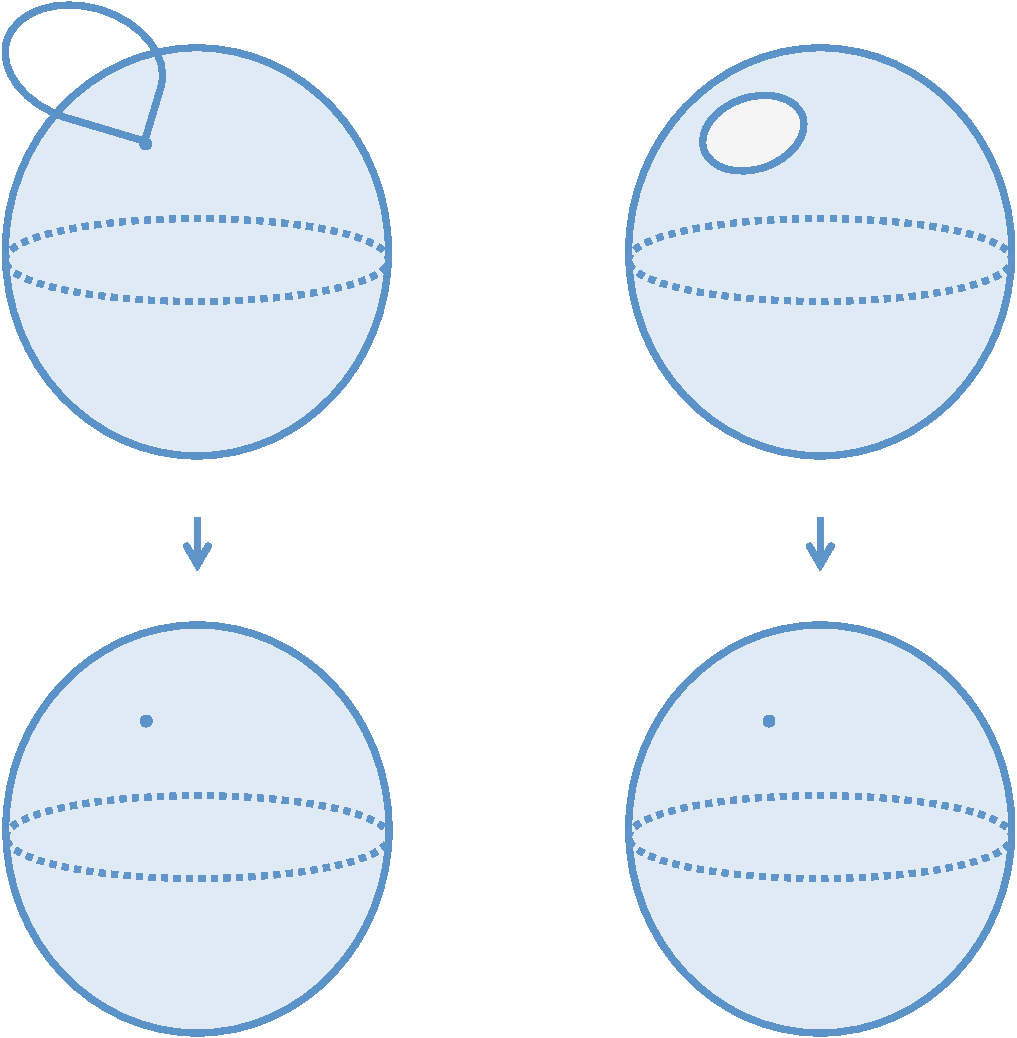
\includegraphics[width=\textwidth]{derived_category_bold.pdf}
    \caption{MacPherson's Motivating Example for the Derived Category}
    \label{fig:derived_category}
\end{figure}

The need for a derived perspective can be stated with one picture. In Figure~\ref{fig:derived_category} two maps are drawn to the two-sphere $S^2$. One is defined on the wedge sum $S^2\vee S^1$ and maps the $S^1$ to a point. The other is defined on the closed disk $\DD^2$ and maps the boundary circle to a point. If one is only allowed to look at the homology of the fiber for both of these maps, they will not be able to tell them apart. The derived category is the universal solution to this problem, as well as many others. 

In the derived category, one does not consider a sheaf in isolation, but rather one considers complexes of sheaves or, alternatively said, sheaves of complexes. In order to solve the problem presented by Figure~\ref{fig:derived_category}, one works with the sheaf of cochains on each fiber, along with their differentials. This transition is formally motivated via an analogy with Taylor series in Section \ref{subsec:taylor}. Injective and projective sheaves are introduced as the basic building blocks for the derived category, just as polynomials are the basis for Taylor series. Because the Alexandrov topology is so simple, we can described explicitly the elementary injective and projective (co)sheaves in Section \ref{subsubsec:elem_inj}. Injective and projective resolutions are then introduced in Section \ref{subsubsec:resolutions}.

Section \ref{subsec:htpy_chain} gives a high-level introduction to the homological algebra techniques necessary to understanding the derived category. The explicitness of cellular sheaves allows us to give concrete examples of what is usually taken on faith when first learning the subject. The notion that maps are unique up to homotopy and that sheaves can be ``quasi''-isomorphic without being isomorphic, are demonstrated in Examples \ref{ex:not_unique} and \ref{ex:quasi_iso}.

The derived definition of cosheaf homology is given in Section \ref{subsec:derived_sheaf_cohom} and the derived definition of sheaf cohomology can be dualized from there or looked up in Shepard's thesis~\cite{shepard}. These definitions should be regarded as the true definition of cosheaf homology and sheaf cohomology. The compactly supported variant, which we call Borel-Moore cosheaf homology, is defined in Section \ref{subsubsec:BM_cosheaf_homology}. The derived functor formalism allows us to resolve the question of invariance under subdivision in Section \ref{subsubsec:subdivision} with considerable ease.

Finally, we exploit the special features of the Alexandrov topology to develop two new theories: sheaf \emph{homology} and cosheaf \emph{cohomology}. Although these theories are invariant under subdivision in the domain of a map, they are not invariant under subdivision in the target of a map. These theories are sensitive to both the cell structure and the embedding. We compute some explicit examples of these theories in Section \ref{subsubsec:sheaf_homology_graphs}.

\section{Taylor Series for Sheaves}
\label{subsec:taylor}

When first learning about the derived perspective a helpful analogy might be the following. We can approximate suitably nice functions around a point via the use of Taylor series:
\[
	f(x)\simeq f(a) + f'(a)(x-a) + \frac{f''(a)}{2!}(x-a)^2+\cdots
\]  
The working physicist or engineer appreciates deeply how by only using a few terms, one can make serious headway into the analysis of integrals or other problems involving $f$.

In similar spirit one might start approximating or ``taking the Taylor series expansion'' of a topological space $X$ via its homotopy or homology groups:
\[
	\pi_0(X,x) \quad \pi_1(X,x) \quad \pi_2(X,x) \quad \cdots \qquad | \qquad \cdots \quad H_2(X) \quad H_1(X) \quad H_0(X)
\]
One should realize that both of these series expansions arise from more fundamental sequences:
\[
	X\to \Omega_x X \to \Omega_x^2 X \to \cdots\qquad | \qquad \cdots \to C_2(X;k)\to C_1(X;k) \to C_0(X;k)
\]
Here $\Omega_x X$ denotes the space of loops in $X$ based at $x$ (and iterated applications thereof) and $C_p(X;k)$ denotes the $p$-chains.

For a sheaf $F$ on a topological space $X$ one also has a similar process. Namely, there is an exact sequence called a \textbf{resolution}
\[
	0 \to F\to I^0 \to I^1 \to I^2 \to \cdots
\]
that when evaluated on an open set $U\subset X$ produces a sequence
\[
	0 \to F(U) \to I^0(U) \to I^1(U) \to I^2(U) \to \cdots
\]
that is exact at $F(U)$ and $I^0(U)$.\footnote{There is no guarantee for exactness at higher terms.} Like the physicist with their Taylor series, one can discard the original sheaf and work solely with the terms in the sequence $I^{\bullet}(U)$. This sequence is a chain complex with potentially interesting cohomology. For each $i$, these cohomologies piece together to provide a pre-sheaf description of the complex of sheaves $I^{\bullet}$ --- the derived replacement for $F$.
\[
	U \rightsquigarrow H^i(I^{\bullet}(U))=:H^i(U;F).
\]
If we specialize to the constant sheaf $F=k_X$, then we obtain another familiar series expansion of the space $X$: the cohomology. However, this series is much more general, as it encodes the cohomology of each open set in $X$. Consequently, even if one embeds $X$ into the contractible cone $CX$, the constant sheaf and its derived replacement will remember the topology on $X$.

However, just as the reason that Taylor series are amenable to analysis because polynomials have simple properties, for general sheaves we must develop an algebraic analogue of a polynomial, which are the injective sheaves.

\subsection{Elementary Injectives and Projectives}
\label{subsubsec:elem_inj}

In this section we consider the basic building blocks of the derived category, which are injective or projective objects. These objects are characterized by universal mapping properties. For cellular sheaves and cosheaves the injectives and projectives can be described explicitly.

\subsubsection{Injectives}
\begin{defn}\index{injective!objects}
 A representation of a small category $I:\cat\to\Vect$ is \textbf{injective} if, for any natural transformation $\eta:A\to I$ and any injection $\iota:A\hookrightarrow B$, there is an extension $\tilde{\eta}:B\to I$ such that $\eta=\tilde{\eta}\circ\iota$. Said using diagrams, they are characterized by the usual universal property:
\[
 \xymatrix{0 \ar[r] & A \ar[r]^{\iota} \ar[d]_{\eta} & B \ar@{.>}[dl]^{\exists \tilde{\eta}} \\ & I &}
\]
\end{defn}

\begin{exr}\label{exr:inj_props}\index{injective!properties}
Use the universal property of an injective representation to prove the following statements:
 \begin{itemize}
  \item Every short exact sequence \[0\to I\to A \to Q \to 0,\] where $I$ is injective, splits, i.e. if $\iota: I\hookrightarrow A$ is an inclusion, then $A\cong I\oplus \cok(\iota)$.
  \item $\prod A_i$ is injective if and only if each $A_i$ is injective.
 \end{itemize}
 We will make use of these properties in Lemma~\ref{lem:inj}.
\end{exr}

For our first example of an injective representation, we consider an injective cell sheaf. These sheaves are supported on the closures of cells.

\begin{defn}\index{sheaf!elementary injective cellular sheaf $[\sigma]^W$}\index{injective!cellular sheaf}
 An \textbf{elementary injective cell sheaf} on $X$ concentrated on $\sigma\in X$ with value $W\in\Vect$ is given by
\begin{equation*}
[\sigma]^W(\tau)=
\begin{cases}
W & \text{if } \tau\leq \sigma,\\
0 & \text{other wise.}
\end{cases}
\end{equation*}
where the only possible non-zero restriction maps are the identity.
\end{defn}

In order to prove that this sheaf is actually injective we introduce an alternative definition of injective sheaves and cosheaves defined on arbitrary posets. This definition makes use of the functors $f_*$ and $f_{\dd}$.

\begin{defn}\index{injective!sheaf on a poset}\index{sheaf!elementary injective on a poset}\index{injective!cosheaf on a poset}\index{cosheaf!elementary injective on a poset}
 Let $i_x:\star \to X$ be the map that assigns to the one element poset the value $x\in X$, i.e. $x=i_x(\star)$. Define the \textbf{elementary injective sheaf} on $x\in X$ with value $W\in\Vect$ to be  $[x]^W=(i_x)_*W$ and the corresponding elementary injective cosheaf to be $\{\hat{x}\}^W:=(i_x)_{\dd}\hat{W}$. 
\end{defn} 

One can see that for cosheaves, the elementary injectives are concentrated on the open stars of cells. To prove these objects are actually injective we make use of the adjunctions already defined.

\begin{lem}
	The sheaf $[x]^W=(i_x)_*W$ and cosheaf $\{\hat{x}\}^W:=(i_x)_{\dd}\hat{W}$ are injective.
\end{lem}
\begin{proof}
	The proof is immediate from the following adjunctions
	\[
		\Hom_{\Shv(X)}(A,(i_x)_*W)\cong \Hom_{\Vect} (A(x),W)
	\]
	\[ 
		\Hom_{\Coshv(X)}(\hat{A},(i_x)_{\dd}\hat{W})\cong \Hom_{\Vect}(\hat{A}(x),\hat{W})
	\]
	and the fact that in the category of vector spaces every object is injective.
\end{proof} 

There is one last lemma that tells us that the considering sheaves of the form $[x]^W$ suffices for understanding all injective sheaves over a cell complex. The proof is presented in~\cite[Thm.~1.3.2, p.19-20]{shepard}, but we will give the direction needed for our derived equivalence proof given in Theorem~\ref{thm:equivalence}.

\begin{lem}[All Injectives are Sums]\label{lem:inj}\index{injective!cellular sheaves are sums}
Let $X$ be the face-relation poset of a cell complex. A sheaf $I$ is injective if and only if it is isomorphic to a one of the form $\oplus_{\sigma}[\sigma]^{V_{\sigma}}$.
\end{lem}
\begin{proof}
One can easily check that the direct sum of elementary injective sheaves is injective, so this proves the `if' direction.

To prove that every injective is isomorphic to a direct sum of injectives --- the `only if' direction --- requires a little work. Assume for induction that every injective sheaf $I$ that is non-zero on at most $k\leq n-1$ cells is isomorphic to $\oplus_{\sigma}[\sigma]^{V_{\sigma}}$. Now consider an injective sheaf that is non-zero on exactly $n$ cells. Let $\sigma$ be a cell of maximal dimension where $I(\sigma)=:V\neq 0$. Since $I$ is zero on all higher cells incidence to $\sigma$, there is a non-zero map $\eta$ from the skyscraper sheaf $S^V_{\sigma}$ to $I$ with $\eta(\sigma)=\id_V$. There is also a non-zero map $\iota:S_{\sigma}^V\to[\sigma]^V$. This gives us a diagram
\[
 \xymatrix{0 \ar[r] & S_{\sigma}^V \ar[r]^{\iota} \ar[d]_{\eta} & [\sigma]^V \ar@{.>}[dl]^{\exists \tilde{\eta}} \\ & I &}
\]
and the implicated existence of a map $\tilde{\eta}:[\sigma]^V\to I$. If $\tau\leq \sigma$, then by the fact that $\tilde{\eta}$ is a sheaf map,
\[
\id_V=\tilde{\eta}(\sigma)\circ \rho^{[\sigma]}_{\sigma,\tau}=\rho^{I}_{\sigma,\tau}\circ \tilde{\eta}(\tau)
\]
the map $\tilde{\eta}$ is injective. By the second property of Exercise~\ref{exr:inj_props}, we can deduce that $I\cong [\sigma]^V\oplus \cok(\tilde{\eta})$. Since $\cok(\tilde{\eta})$ is zero wherever $I$ is and also zero on $\sigma$, it is non-zero on at most $n-1$ cells and the induction hypothesis applies. The zero sheaf is clearly equal to a direct sum of elementary injectives with the zero vector space, which checks the base case, completing the induction.
\end{proof}

\subsubsection{Projectives}

There is a dual universal object that is called projective.
\begin{defn}\index{projective!objects}
 A representation of a small category $P$ is \textbf{projective} if for any natural transformation $\epsilon:P\to A$ and any surjection $\pi:B\twoheadrightarrow A$, there is a map $\tilde{\epsilon}:P\to B$ such that $\epsilon=\pi\circ \tilde{\epsilon}$. Said using diagrams:
\[
 \xymatrix{ & P\ar[d]^{\epsilon} \ar@{.>}[dl]_{\exists \tilde{\epsilon}} & \\ B \ar[r]_{\pi} &  A \ar[r] & 0}
\]
\end{defn}

As before, we have some dual consequences:
\begin{itemize}\index{projective!properties}
 \item Every short exact sequence \[0\to A \to B \to P \to 0\] where $P$ is projective, splits.
 \item $\oplus B_i$ is projective if and only if each $B_i$ is projective.
\end{itemize}

Since the adjunctions will be our guide we make the following definitions.

\begin{defn}\index{projective!sheaf on a poset}\index{sheaf!elementary projective on a poset}\index{projective!cosheaf on a poset}\index{cosheaf!elementary projective on a poset}
 Let $i_x:\star \to X$ be the map that assigns to the one element poset the value $x\in X$, i.e. $x=i_x(\star)$. Define the elementary projective sheaf on $x\in X$ with value $W\in\Vect$ to be  $\{x\}^W=(i_x)_{\dd}W$ and the corresponding elementary projective cosheaf to be $[\hat{x}]^W:=(i_x)_{*}\hat{W}$. 
\end{defn}

We leave it to the reader to check that these objects are actually projective.

\subsubsection{Mapping Identities}
\index{injective!mapping identities for (co)sheaves}
\index{projective!mapping identities for (co)sheaves}

Before moving on to the derived definition of sheaf cohomology, we record some useful identities that should be evident from the definition and the adjunctions.

\begin{equation*}
 \Hom_{\Shv}([\tau]^U,[\sigma]^W)=
\begin{cases}
 \Hom_{\Vect}(U,W) & \text{if } \sigma \leq \tau, \\
0 & \text{o.w.}
\end{cases}
\end{equation*}

\begin{equation*}
 \Hom_{\Shv}(\{\tau\}^U,\{\sigma\}^W)=
\begin{cases}
 \Hom_{\Vect}(U,W) & \text{if } \sigma \leq \tau, \\
0 & \text{o.w.}
\end{cases}
\end{equation*}

\begin{equation*}
 \Hom_{\Coshv}([\hat{\sigma}]^W,[\hat{\tau}]^U)=
\begin{cases}
 \Hom_{\Vect}(W,U) & \text{if } \sigma \leq \tau, \\
0 & \text{o.w.}
\end{cases}
\end{equation*}

\begin{equation*}
 \Hom_{\Coshv}(\{\hat{\sigma}\}^W,\{\hat{\tau}\}^U)=
\begin{cases}
 \Hom_{\Vect}(W,U) & \text{if } \sigma \leq \tau, \\
0 & \text{o.w.}
\end{cases}
\end{equation*}

\subsection{Injective and Projective Resolutions}
\label{subsubsec:resolutions}
\index{injective!resolutions}\index{projective!resolutions}

As promised, we aim to prove every sheaf has a resolution by injective sheaves. This follows from the following claim, which we now prove. Although this theorem is true for general spaces, we work with Alexandrov spaces arising as posets as usual.

\begin{clm}
	Every sheaf $F:X\to\Vect$ on a poset $(X,\leq)$ possibly of infinite size, $F$ admits an inclusion into an injective sheaf. Dually, every cosheaf admits is surjected onto by a projective cosheaf.
	\[
		0 \to F \to I
	\]
\end{clm}
\begin{proof}
	We construct $I$ explicitly. It is given by
	\[
		0 \to F \to I:=\prod_x [x]^{F(x)} = \prod_x (i_x)_*F(x).
	\]
	The map to $I$ is defined easily using the standard adjunctions
	\[
		\iota\in \Hom(F,\prod_x(i_x)_*F(x))\cong \prod_x \Hom(F,\prod_x(i_x)_*F(x)) \cong \prod_x \Hom(F(x),F(x)) \ni \prod_x \id_{F(x)}.
	\]
	We encourage the reader to describe this map is explicitly, by seeing how a single $\id_{F(x)}$ traces through this adjunction, which we'll call $\iota_x\in \Hom(F,(i_x)_*F(x))$.
	
	Similarly, for a cosheaf $\hF:X^{op}\to\Vect$ on an Alexandrov space we could have built a projective surjection by taking
	\[
	 \hat{P}_0:=\bigoplus_{x} (i_x)_*\hF(x) \to \hF \to 0
	\]
	where the map $\pi_0:P_0\to \hF$ is gotten through the corresponding adjunction for cosheaves and using the contravariance of $\Hom$ in the first slot
	\[
		\Hom(\bigoplus_{x} (i_x)_*\hF(x),\hF)\cong \prod \Hom((i_x)_*\hF(x),\hF)\cong \prod \Hom(\hF(x),\hF(x)).
	\]
\end{proof}

\begin{cor}
	Every sheaf $F:X\to\Vect$ has an injective resolution. Dually, every cosheaf $\hF:X^{op}\to\Vect$ has a projective resolution.
\end{cor}
\begin{proof}
	Since cokernels exist in the category of sheaves by taking element-by-element quotients and by iteratively applying the claim, we obtain an injective resolution of $F$:
	\[
	 \xymatrix{F \ar[r]^{\iota^0} & I^0 \ar[rd]_{\pi_0} \ar[rr]^{\iota^1=j_1\pi_0} & & I^1 \ar[rr]^{\iota^2=j_2\pi_1} \ar[rd]_{\pi_1} & & I^2 &\cdots \\
		      & & \cok(\iota^0) \ar[ru]_{j_1} & & \cok(\iota^1) \ar[ru]_{j_2} & &\cdots }
	\]
	
	Iterating the analogous process for projective cosheaves, replacing kernels where one sees cokernels above, one obtains an exact sequence of cosheaves called the \textbf{projective resolution} of $\hF$:
	\[
	 \cdots \hat{P}_2 \to \hat{P}_1 \to \hat{P}_0 \to \hF \to 0.
	\]
\end{proof}

These exact sequences can be used to replace $F$ or $\hF$ in a suitable sense, defined by the derived category. Before moving onto that discussion, we note one interesting point.

\begin{prop}
 The length of injective resolution of any sheaf $F\in\Shv(X)$ is bounded by the length of longest chain in the poset. In particular for $X$ a cell complex, it is bounded by the dimension.
\end{prop}
\begin{proof}
 Pick a maximal ordered subset in $X$ and consider its top element, say $x'$, then $I^0(x')=F(x')$ since nothing is larger than $x'$. The cokernel sheaf of $\iota^0$ evaluated on $x'$ is then $\cok(\id:F(x')\to F(x'))=0$. So for any maximally ordered chain in $X$, $I^1$ is zero on the top-most element. Arguing inductively finishes the proof.
\end{proof}

\section{The Derived Category and Homotopy Theory of Chain Complexes}
\label{subsec:htpy_chain}

The purpose of the derived category is to replace the category of sheaves with a category of complexes where certain operations are more natural. We have already shown that one can replace a sheaf by its injective resolution and a cosheaf by its projective resolution. This will define our derived replacement on the level of objects, but we have not yet shown how a map of sheaves or cosheaves induces a map on the level of resolutions. 

If $\phi:\hF\to\hG$ is a map of cosheaves, then it can be checked from the universal properties of projective objects, that this induces a map of complexes
\[
	\xymatrix{ \cdots & \hat{P}_2 \ar[r] \ar@{.>}[d]^{\phi_2} & \hat{P}_1 \ar[r] \ar@{.>}[d]^{\phi_1} & \hat{P}_0 \ar[r] \ar@{.>}[d]^{\phi_0} & \hF \ar[d]^{\phi} \ar[r] & 0\\ \cdots & \hat{Q}_2 \ar[r] & \hat{Q}_1 \ar[r] & \hat{Q}_0 \ar[r] & \hG \ar[r] & 0}
\]
where all the squares in sight commute. For a hint on how to see this, consider the composite map $\hat{P}_0\to\hF\to\hG$ and let $\hG=A$ and $B=\hat{Q}_0$ in the definition of the universal property defining a projective object. This induces our first map $\hat{P}_0\to\hat{Q}_0$. To get the next, all important step, one must recognize that having maps from $\hat{P}_0\to \hat{Q}_0$ and $\hF\to\hG$ induces maps between the kernels of the map $\hat{P}_0\to\hF$ and $\hat{Q}_0\to\hG$. Since $\hat{Q}_1$ surjects onto the kernel of the latter map repeating the initial argument provides a map from $\hat{P}_1$ to $\hat{Q}_1$. This shows that the projective replacement of cosheaves is functorial.

Aside from functoriality, there is one more snag that needs to be mentioned: For a sheaf or a cosheaf it is possible that the choice of injective or projective resolution is not unique. If one really wants to use these as replacements for the original sheaf or cosheaf, there must be a strong relationship between these two complexes. This is best seen by specializing the functoriality discussion above to the case $\phi=\id$.
\[
	\xymatrix{ \cdots & \hat{P}_2 \ar[r] \ar@{.>}[d]^{\phi_2} & \hat{P}_1 \ar[r] \ar@{.>}[d]^{\phi_1} & \hat{P}_0 \ar[r] \ar@{.>}[d]^{\phi_0} & \hF \ar[d]^{\id} \ar[r] & 0\\
	\cdots & \hat{Q}_2 \ar[r] & \hat{Q}_1 \ar[r] & \hat{Q}_0 \ar[r] & \hF \ar[r] & 0}
\]
The resulting map of complexes need not be a term-by-term isomorphism with all squares in sight commuting, but rather a more general notion must be substituted, namely the definition of chain homotopy. Before giving that, let us give an example.

\begin{ex}[Non-Unique Projective Resolutions]
	Let us work again over our test space of the closed unit interval $X=[0,1]$ stratified as $x=0$, $y=1$ and $a=(0,1)$. The constant cosheaf $\hat{k}_X$ is then modeled as
	\[
		\xymatrix{ & \ar[ld]_1 k \ar[rd]^1 & \\ k & & k}
	\]
	Revisiting the definition of the elementary projective cosheaves, there is one obvious projective resolution because the constant cosheaf on this stratification of the unit interval is already projective, so we have the identity map
	\[
		\hat{P}_{\bullet}: \qquad [\hat{a}] \to \hat{k}_X.
	\]
	On the other hand, following blindly the prescription provided for computing the projective resolution of an arbitrary cellular cosheaf would have lead us to the following ``canonical'' resolution:
	\[
		\hat{Q}_{\bullet}: \qquad [\hat{x}]\oplus [\hat{y}]\to [\hat{a}]\oplus [\hat{x}]\oplus [\hat{y}] \to \hat{k}_X
	\]
\end{ex}

\begin{defn}[Chain Homotopy]\index{Cochain@(co)chain complex!homotopy}
	Suppose $(A^{\bullet},d_A)$ and $(B^{\bullet},d_B)$ are two (cohomological) chain complexes and $\phi^{\bullet}$ and $\psi^{\bullet}$ are two chain maps, then \textbf{a chain homotopy} $h^{\bullet}$ is a chain map $h^i:A^{i}\to B^{i-1}$
	\[
		\xymatrix{\cdots\ar[r] & A^{i-2} \ar[d] \ar[r] & \ar[ld] A^{i-1} \ar[r] \ar[d]^{\psi^{i-1}}_{\phi^{i-1}} & \ar[ld] A^i \ar[r] \ar[d]^{\psi^i}_{\phi^i} & \ar[ld] A^{i+1} \ar[d]^{\psi^{i+1}}_{\phi^{i+1}} \ar[r] & \cdots \\
		\cdots \ar[r] & B^{i-2} \ar[r] & B^{i-1} \ar[r] & B^i \ar[r] & B^{i+1} \ar[r] & \cdots}
	\]
	such that 
	\[ 
		\phi^i-\psi^i=h^{i+1}d^i_A+d^{i-1}_Bh^i.
	\]
	In which case we say that $\phi\sim\psi$ are \textbf{chain homotopic}. 
	
	Consider now two chain maps $\phi:A^{\bullet}\to B^{\bullet}$ and $\psi:B^{\bullet}\to A^{\bullet}$, such that
	\[
		\phi\circ\psi \sim \id \qquad \mathrm{and} \qquad \psi\circ\phi \sim \id
	\]
	then one says $A^{\bullet}$ and $B^{\bullet}$ are \textbf{chain homotopy equivalent}.
\end{defn}

\begin{ex}[Non-unique, but equivalent]\label{ex:not_unique}
	Consider again the case of the two different projective resolutions of the constant sheaf $\hat{k}_X$ on the closed unit interval. On the one hand the composite
	\[
		\xymatrix{ 0 \ar[d] \ar[r] & [\hat{a}] \ar[d] \\
		[\hat{x}]\oplus [\hat{y}] \ar[d] \ar[r] & [\hat{x}]\oplus [\hat{a}]\oplus [\hat{y}] \ar[d] \\
		0 \ar[r] & [\hat{a}] }
	\]
	is clearly the identity on $\hat{P}_{\bullet}$, but the composite
	\[
		\xymatrix{
		[\hat{x}]\oplus [\hat{y}] \ar[d] \ar[r] & [\hat{x}]\oplus [\hat{a}]\oplus [\hat{y}] \ar[d] \\
		 0 \ar[d] \ar[r] & [\hat{a}] \ar[d] \\
		[\hat{x}]\oplus [\hat{y}] \ar[r] & [\hat{x}]\oplus [\hat{a}]\oplus [\hat{y}] }
	\]
	cannot possibly be the identity because one map factors through zero. However, if we employ a self-homotopy of $\hat{Q}_{\bullet}$ by defining a homotopy for the only possible degree to be
	\[
		h^0:[\hat{a}]\oplus[\hat{x}]\oplus[\hat{y}] \to  [\hat{x}]\oplus[\hat{y}]
	\]
	which is zero on the $a$ component and the identity elsewhere. One can then check that this defines a homotopy between the identity map and the map indicated in the second composite.
\end{ex}

The conclusion from the example should be that although one can use different projective resolutions, the choice is irrelevant up to homotopy. The derived category should not be able to discriminate between them. As such, we make the following definitions.

\begin{defn}\index{category!C@$C^b(\aat)$ of chain complexes}\index{category!K@$K^b(\aat)$ homotopy category of chain complexes}\index{H@$K^b(\aat)$ homotopy category of chain complexes}
	Let $\aat$ be an abelian category, such as the category of sheaves or cosheaves. The \textbf{category of chain complexes} in $\aat$, written $C^b(\aat)$ has objects that are chain complexes and morphisms that are chain maps.
	
	The \textbf{homotopy category of complexes} $K^b(\aat)$ of an abelian category $\aat$ has the same objects as $C^b(\aat)$, but where we have identified chain homotopic maps.
\end{defn}

\begin{defn}\index{Derived@$D^b(\aat)$ derived category}\index{category!Derived@$D^b(\aat)$ derived category}
	For $\aat=\Shv(X)$ we define the \textbf{bounded derived category of sheaves} $D^b(\Shv(X))$ to be $K^b(\mathrm{Inj}-\Shv(X))$ the homotopy category that uses only complexes of injective sheaves. 
	
	Similarly, for $\aat=\Coshv(X)$, we define the \textbf{bounded derived category of cosheaves} $D^b(\Coshv(X))$ by $K^b(\mathrm{Proj}-\Coshv(X))$ where complexes of projective cosheaves are used instead.
\end{defn}

This definition, is an equivalent reformulation of another definition of the derived category. This other perspective is built on the foundational notion of a quasi-isomorphism, which is in turn built on the idea of a cohomology sheaf or homology cosheaf.

\begin{defn}
	Suppose we are given a complex of cellular sheaves
	\[
		(F^{\bullet},d^{\bullet}): \qquad \cdots \to F^{i-1} \to F^{i} \to F^{i+1} \to \cdots,
	\]
	i.e. for each cell $\sigma$ we have a complex of vector spaces. For each $i$ we can define the $i$th \textbf{cohomology sheaf} as the assignment
	\[
		\cohomsheaf^i(F^{\bullet}): \qquad \sigma \rightsquigarrow H^i(F^{\bullet}(\sigma))
	\]
	which is a cellular sheaf. The restriction maps being defined as the induced map on cohomology for the chain map $F^{\bullet}(\sigma)\to F^{\bullet}(\tau)$ for $\sigma\leq\tau$. 
	
	Considering all $i$ at once defines a functor from the category of complexes of sheaves and the category of graded sheaves (sheaves of graded vector spaces with level preserving restriction maps)
	\[
		\cohomsheaf^*: C^b(\Shv(X))\to \Shv(X;\mathrm{gr}\Vect) \qquad F^{\bullet} \rightsquigarrow \bigoplus_i \cohomsheaf^i(F^{\bullet}).
	\]
	There are completely dual notions of \textbf{homology cosheaves}, where we generally use homological indexing and notation $(\hF_{\bullet},\partial_{\bullet})$.
\end{defn}

\begin{defn}[Quasi-Isomorphisms]\index{quasi-isomorphism}
	A map of complexes of sheaves (or cosheaves) $\alpha^{\bullet}:F^{\bullet}\to G^{\bullet}$ such that the induced map
	\[
		\cohomsheaf(\alpha^{\bullet}):\cohomsheaf^i(F^{\bullet})\to \cohomsheaf^i(G^{\bullet})
	\]
	is an isomorphisms for every $i$, is called a \textbf{quasi-isomorphism}.
\end{defn}
	
The term ``quasi-isomorphism'' reflects the fact that if $\alpha^{\bullet}:F^{\bullet}\to G^{\bullet}$ is a quasi-isomorphism, then there does not always exist an inverse map $\beta^{\bullet}$ that gives the identity, or even chain homotopic to the identity, any map back may simply not exist.
	
\begin{ex}\label{ex:quasi_iso}
	Consider again the unit interval $X=[0,1]$ decomposed into two vertices $x$ and $y$ and an open interval $a$. Consider the stalk sheaf $S_a$ that assigns $k$ to $a$ and is zero everywhere else. It's injective resolution defines a chain map
	\[
	\xymatrix{ 0\ar[r] \ar[d] & S_a \ar[r] \ar[d] & 0 \ar[d] \\
	0  \ar[r] & [a] \ar[r] & [x]\oplus [y] }
	\]
	which is a quasi-isomorphism. However, there does not exist a map of sheaves $[a]\to S_a$.
\end{ex}

The slogan most commonly associated with the derived category is that one ``formally inverts the quasi-isomorphisms.'' This is formalized by the process of localizing categories. Namely, if $Q$ is a collection of morphisms in $\bat$ that is closed under certain operations, then we can consider the following universal problem: suppose $L:\bat\to\cat$ is a functor such that if $\alpha\in Q$, then $L(\alpha)$ is an isomorphism, then every such functor factors through the \textbf{category localized at $Q$}, written $\bat[Q^{-1}]$.
\[
	\xymatrix{\bat \ar[rr]^L \ar[rd] & & \cat \\
	& \bat[Q^{-1}] \ar@{.>}[ur]_{\exists} & }
\]
An alternative approach to the derived category of an abelian category $\aat$ is to define
\[
	D(\aat):= K(\aat)[Q^{-1}] \qquad Q=\{\mathrm{quasi-isomorphisms}\}
\]
where we have removed the boundedness hypothesis.

One then proves the following claim to re-obtain the definition we provided here
\begin{thm}[\cite{aluffi} Thm 6.7]\label{thm:proj_or_inj}
	Suppose $A$ is an abelian category with enough projectives, then $D^-(A)\cong K^-(P)$ where $P$ denotes projective objects of $A$. Similarly, if $A$ has enough injectives then $D^+(A)\cong K^+(I)$ where $I$ denotes injective objects of $A$.
\end{thm}


\section{The Derived Definition of Cosheaf Homology and Sheaf Cohomology}
\label{subsec:derived_sheaf_cohom}

We are now in a position to give the derived definition of cosheaf homology and show that it agrees with the computational formula provided earlier. This discussion can be dualized and readily found in the literature. The proof that the formula for sheaves computes the cohomology as defined by taking an injective resolution and applying $\Gamma(X;-)=p_*$ can be found in~\cite{shepard} pp. 28-29. Let's more or less repeat the proof for cellular cosheaves since it is nowhere in the literature.

\begin{defn}\index{Left@$Lf_*$ left derived pushforward}
	Given a cosheaf $\hF$ on $X$ we define the \textbf{left derived pushforward} along $f:X\to Y$ by taking a projective resolution and applying pushforward term by term:
	\[
		Lf_*\hF:=f_*P_{\bullet}.
	\]
	We define the $i$th derived functor by
	\[
		L_if_*\hF:= \cohomsheaf_i(f_*P_{\bullet}).
	\]
	In the special case where $f=p:X\to\star$ we write
	\[
		H_i(X;\hF):=L_ip_*\hF
	\]
	for the $i$th cosheaf homology group of $\hF$.
\end{defn}

We now aim to prove the following theorem.
\begin{thm}\index{cosheaf!cellular homology!Left@$Lf_*$ left derived pushforward}
 Let $p:X\to\star$ be the constant map and $\hat{F}$ a cellular cosheaf on $X$. Then the left derived functors of $p_{*}$ agree with the computational formula for homology, i.e. $L_i p_{*}\hat{F}=H_i(X;\hat{F})$.
\end{thm}
\begin{proof}
Begin with a projective resolution of $\hat{P}_{\bullet}\to\hat{F}$ and then take cellular chains of each cosheaf to obtain the following double complex:
\[
 \xymatrix{ & \vdots & \vdots & \vdots & \\
\cdots &  C_1(X;\hat{P}_1) \ar[r]\ar[d] & C_1(X;\hat{P}_0) \ar[r]\ar[d] & C_1(X;\hat{F}) \ar[r]\ar[d] & 0 \\
\cdots & C_0(X;\hat{P}_1)\ar[r]\ar[d] & C_0(X;\hat{P}_0)\ar[r]\ar[d] & C_0(X;\hat{F})\ar[r]\ar[d] & 0 \\
\cdots & \colim \hat{P}_1 \ar[r] \ar[d]& \colim \hat{P}_0\ar[r]\ar[d] & \colim \hat{F}\ar[r]\ar[d] & 0 \\
& 0 & 0 & 0 &}
\]

Now we make use of the following two observations, which dualize~\cite[Thm. 1.3.10, 1.4.1]{shepard}.
\begin{lem}
 For $\hat{P}$ a projective cosheaf 
$$H_p(C_{\bullet}^{BM}(X;\hat{P}))\cong H_p(C_{\bullet}(X;\hat{P}))\cong 0$$ for $p>0$.
\end{lem}
\begin{proof}
 Observe that we can assume that $\hat{P}$ is an elementary projective co-sheaf with value $\RR$, i.e. $[\hat{\sigma}]$, since $C_{\bullet}^{BM}(X;\oplus A_i)=\oplus C_{\bullet}^{BM}(X;A_i)$.

Everything follows from the following consequence of our definition of a cell complex: In the one-point compactification of $X$, the closure of any cell $\sigma\in X$, call it $|\bar{\bar{\sigma}}|$, has the homeomorphism type of a closed $k$-simplex.

$C_{\bullet}(X;[\hat{\sigma}])$ is the chain complex that computes the cellular homology of $Y=|\{\tau\leq \sigma|\bar{\tau}\,\mathrm{is}\,\mathrm{compact}\}|$, which is a closed $k$-simplex minus the star of a vertex. On the other hand, $C^{BM}_{\bullet}(X;[\hat{\sigma}])$ is equal to the chain complex calculating the cellular homology of $|\bar{\bar{\sigma}}|$ except in degree zero if $|\bar{\sigma}|$ is not compact. Notice that $H_1$ for both of these complexes is the same, as $|\bar{\sigma}|$ and $|\bar{\bar{\sigma}}|$ are simply connected. This proves the claim.
\end{proof}

\begin{lem}
 For any cellular cosheaf $\hat{F}$ on a cell complex $X$ we have that $$\colim \hat{F}\cong\cok(C_1(X;\hat{F})\to C_0(X;\hat{F})).$$
\end{lem}
\begin{proof}
 First let us prove that taking the coproduct of $\hat{F}$ over all the cells obtains a vector space that surjects onto the colimit. As part of the definition of $\colim \hat{F}$ is a choice of maps $\psi_{\sigma}:\hat{F}(\sigma)\to\colim \hat{F}$.  Let $\Psi=\oplus \psi_{\sigma}:\oplus \hat{F}(\sigma)\to \colim \hat{F}$, now consider the factorization of this map through the image:
\[
 \xymatrix{\oplus \hat{F}(\sigma) \ar[rr]^{\Psi} \ar[rd] & & \colim \hat{F} \\
& \im \Psi \ar[ru]^j &}
\]
Now we can use the $\im \Psi$ to define a new co-cone over the diagram $\hat{F}$ simply by pre-composing the factorized map with the inclusions $i_{\sigma}:\hat{F}(\sigma)\to\oplus \hat{F}(\sigma)$. Since the colimit is the initial object in the category of co-cones, there must be a map $u:\colim \hat{F}\to \im \Psi$ and thus $u\circ j=\id$ since there is only one map $\colim\hat{F}\to\colim\hat{F}$.

Now observe that $C_0(X;\hat{F})=\oplus \hat{F}(v_i)$ surjects onto the colimit of $\hat{F}$ by virtue of the fact that since every cell $\sigma\in X$ has at least one vertex as a face, the map $\Psi$ factors through $\oplus \hat{F}(v_i)$. Thus there is a surjection from $\Psi':C_0(X;\hat{F})\to \colim\hat{F}$. Notice that by universal properties of the cokernel of $\partial_0:C_1(X;\hat{F})\to C_0(X;\hat{F})$ it suffices to check that $\Psi'\circ\partial_0=0$. However, this is clear since every $e$ edge has two vertices $v_1$ and $v_2$ (we've discarded all those edges without compact closures), then we need only check the claim for each diagram of the form
\[
 \xymatrix{ & \hat{F}(e) \ar[ld]_{r_{e,v_1}} \ar[rd]^{r_{e,v_2}} & \\
\hat{F}(v_1) & & \hat{F}(v_2)}
\]
where it is clear that the colimit can be written as $\hat{F}(v_1)\oplus \hat{F}(v_2)$ modulo the equivalence relation $(r_{e,v_1}(w),0)\simeq (0,r_{e,v_2}(w))$, i.e. $\partial_0|_e(w)=(-r_{e,v_1}(w),r_{e,v_2}(w))\simeq(0,0)$.
\end{proof}

From these two theorems we can conclude that the columns away from the chain complex of $\hat{F}$ are exact and thus $\mathrm{Tot}_{\bullet}(C_i(X;\hat{P}_j))$ induces quasi-isomorphisms between $\colim \hat{P}_{\bullet}$ and $C_{\bullet}(X;\hat{F})$. We have thus established the theorem.
\end{proof}

\subsection{Borel-Moore Cosheaf Homology}
\label{subsubsec:BM_cosheaf_homology}
\index{Borel-Moore cosheaf homology}\index{cosheaf!cellular!Borel-Moore homology}
\begin{defn}\label{defn:BM_cosheaf_homology}
 Suppose $\hF$ is a cellular cosheaf. Define $\Gamma^{BM}(X;F)$ to be the colimit of the diagram extended over the one-point compactification of $X$ where we define $\hF(\infty)=0$. Alternatively said we look at the inclusion $j:X\to X\cup\{\infty\}$ and define
\[
	\Gamma^{BM}(X;\hF):=p_*j_{\dd}\hF.
\]
Another possible definition is to dualize a cellular cosheaf of finite-dimensional vector spaces to a cellular sheaf by post-composing $\hF:X\to\Vect$ with $\Hom_{\vect}(-,k)$, apply $p_!$ and then dualize back.
\end{defn}

\begin{rmk}[Functoriality]
	The definitions that involve the one-point compactification are deficient in the following way. A map of cell complexes $f:X\to Y$ does not necessarily extend to a map between the one-point compactifications. It is for this reason that for functoriality, the definition using $p_!$ is preferred.
\end{rmk}

Now we can prove that the formula provided calculates the Borel-Moore homology of a cosheaf $\hat{F}$ by establishing the following lemma:

\begin{lem}\label{lem:BM_cosheaf_homology}
 For any cellular cosheaf $\hat{F}$ on a cell complex $X$ we have that $\Gamma^{BM}(X;\hat{F})\cong \cok(C_1^{BM}(X;\hat{F})\to C^{BM}_0(X;\hat{F}))$.
\end{lem}
\begin{proof}
 The proof above goes through until the last argument. Now we have edges $e$ with only one vertex. However, by extending and zeroing out at infinity to get that the colimit of
\[
 \xymatrix{ & \hat{F}(e) \ar[ld]_{r_{e,v}} \ar[rd]^0 & \\
\hat{F}(v) & & \hat{F}(\infty)=0}
\]
is exactly equal to the co-equalizer of $r_{e,v}:\hat{F}(e)\to F(v)$ and the zero morphism, i.e. the cokernel.
\end{proof}

\subsection{Invariance under Subdivision}
\label{subsubsec:subdivision}
\index{Borel-Moore cosheaf homology!invariance under subdivision}\index{cosheaf!cellular!Borel-Moore homology under subdivision}

Now we take up the question of invariance under subdivision by applying the derived perspective. For convenience, we work with sheaves, but the reasoning can be dualized.

\begin{defn}
 Suppose $F$ is a sheaf on $X$ and $s:X'\to X$ is a subdivision of $X$, then we define the subdivided sheaf $F':=s^*F$.
\end{defn}

For an example, let $X$ be the unit interval $[0,1]$ stratified in the obvious way with $x=0$, $y=1$ and $a=(0,1)$. Now consider a sheaf $F$ on $X$. We will want to investigate what happens to this sheaf as we subdivide the space. In this example, the barycentric subdivision of $X$ produces a space $X'$ with a third vertex $\bar{a}$ and two edges $a_x$ and $a_y$. The obvious way of defining a subdivided sheaf is to define $F'(\bar{a})=F'(a_x)=F'(a_y)=F(a)$ where we use the identity map for the two new restriction maps. Observe that if $F$ is the elementary injective sheaf $[a]$, then $F'$ is \emph{not} an injective sheaf, yet nevertheless $F'$ and $F$ have isomorphic cohomology.

More generally we are concerned with the following diagram of spaces (posets)
\[
 \xymatrix{X' \ar[rr]^s \ar[rd]_{p_{X'}} & & X\ar[ld]^{p_X}\\
	      &\star&}
\]
and the induced functors on sheaves. For example, if we analyze the ordinary pushforward functor, then we would obtain the following result, which is a simplified proof of one found in~\cite[Thm. 1.5.2]{shepard}:

\begin{thm}\label{thm:subdivision}
 Suppose $F$ is a sheaf on $X$ and $X'$ is a subdivision of $X$, then
\[
 H^{\bullet}(X;F)\cong H^{\bullet}(X';F')
\]
\end{thm}
\begin{proof}
Observe that since $p_{X'}=p_X\circ s$, then $(p_{X'})_*=(p_X)_*\circ s_*$. Now recall $$(p_{X'})_*F'=(p_{X'})_*s^*F=(p_{X})_*\circ s_* s^* F.$$ 
The question then boils down to understanding the relationship between $s_*s^*F$ and $F$. Unraveling the definition reveals
\begin{eqnarray*}
 s_*s^*F(y) & = &\varprojlim \{s^*F(x) | s(x)\geq y\} \\
&=&\varprojlim \{F(s(x)) | s(x)\geq y\} \\
(\mathrm{surjectivity})&=&\varprojlim \{F(x) | x\geq y\} \\
(\mathrm{sheaf-axiom})&=& F(U_y) \\
&=& F(y)
\end{eqnarray*}
So we have that for the subdivision map $s_*s^*F\cong F$ and as a consequence
$$(p_{X'})F'\cong p_X F.$$
Now we can just take the associated right derived functors to obtain the result.
\end{proof}

\section{Sheaf Homology and Cosheaf Cohomology}
\label{subsec:sheaf_homology}
\index{sheaf!homology, cellular}\index{cosheaf!cohomology, cellular}

There is a surprising symmetry in the land of cellular sheaves and cosheaves, which is unique to the land of Alexandrov spaces and deserves to be explored. Contrary to the existence of enough injective sheaves, which for general sheaves is gotten as a consequence of the target category, e.g. $\Ab,\Vect$, etc., the existence of enough projective sheaves is driven by the underlying topology of the space.

\begin{prop}
 Suppose $X$ is a topological space with the property that there is a point $x\in X$ such that for every open neighborhood $U\ni x$ there is a strictly smaller open neighborhood $V\subset U$. Then the category of sheaves on $X$ does not have enough projectives.\footnote{The author would like to acknowledge the contributions of Valery Alexeev, David Treumann, and Jon Woolf on mathoverflow in regards to this question.}
\end{prop}
\begin{proof}
 Consider the map $i:x\hookrightarrow X$ and the sheaf $i_*k$. Suppose it has a projective resolution, i.e. a projective sheaf $P$ and a surjection $P\to i_*k$. Now let's examine this map evaluated on an open set $U\ni x$. By assumption there is another open set $V\subset U$ and we can put the constant sheaf extended by zero on $V$, denote the inclusion by $j:V\hookrightarrow X$. Note that we have the following diagram of sheaves
\[
 \xymatrix{j_!\tilde{k}_V \ar[r] & i_*k \ar[r] & 0\\ & P \ar@{.>}[lu] \ar[u] &}
\]
whose value on the open set $U$ is
\[
 \xymatrix{j_!\tilde{k}_V(U)=0 \ar[r] & i_*k(U)=k \ar[r] & 0\\ & P(U) \ar@{.>}[lu] \ar[u] &}
\]
so in particular the surjection must factor through zero --- a contradiction.
\end{proof}

Contrary to sheaves on manifolds and other Hausdorff spaces, cellular sheaves are can be viewed as sheaves on finite posets and as such do not suffer from the above argument. In fact, computing a projective resolution is as easy as computing injective resolutions. To see how this goes recall we need to find a projective sheaf that surjects onto our sheaf of interest. 
\[
 P^0:=\oplus_{\sigma\in X} \{\sigma\}^{F(\sigma)} \to F \to 0
\]
 serves nicely and by finding the kernel sheaf (which is easier to understand than cokernels!) and then iterating this process will obtain a projective resolution
\[
 \cdots P^{-3}\to P^{-2} \to P^{-1} \to P^0 \to F \to 0.
\]

This motivates the following definitions:
\begin{defn}
 Given a cellular sheaf, we can construct its projective resolution $P_{\bullet}\to F$, calculate colimits of $P_{\bullet}$ and take the cohomology of the resulting complex of vector spaces. Assuming $F$ was in degree zero, this will be concentrated in negative degree and we define the \textbf{homology of a cellular sheaf} $F$ to be $H_i(X;F):=H^{-i}(p_{\dd}P_{\bullet})$.

Similarly we define the \textbf{cohomology of a cellular cosheaf} $\hat{F}$ by taking its injective resolution $\hat{I}^{\bullet}$, and taking limits, i.e. $H^i(X;\hat{F})=H^i(\hat{p}_*\hat{I}^{\bullet})$.
\end{defn}

The reasons for it's apocryphal nature are many:
\begin{enumerate}
 \item Only for (co)sheaves over finite spaces are there enough projectives and enough injectives.
 \item Spaces for which there is not a fixed $n$ so that every cell $\sigma$ contains in its star a cell $\tau$ such that $\dim\tau=n$ cannot hope to have the same computational formula for (co)homology because we can't treat the colimit (in the case of a sheaf) as a quotient object of $\oplus_{\dim\tau=n} F(\tau)$ and dually for limits of cosheaves.
 \item This defect, which is measured by the difference of $H^n(X;F)$ and $\colim F$, is only the first in a series of obstructions that appear to detect whether $X$ is a cell structure on a manifold.
\end{enumerate}

The evidence for the last two observations is further solidified in view of the following theorem.

\begin{thm}\label{thm:mfld_sheaf_cosheaf}\index{duality!over a manifold}
 Suppose $F$ is a cellular sheaf on a triangulated closed $n$-manifold $X$, then $F$ defines a cellular cosheaf on the dual triangulation and moreover all the homologies and cohomologies of both agree.
\end{thm}
\begin{proof}
 This is a consequence of the following simple observation:
\[
 \xymatrix{F(\sigma^i) \ar[r]^{\rho_{\sigma,\tau}} \ar@{~>}[d] & F(\tau^{i+1}) \ar@{~>}[d] \\
\hF(\tilde{\sigma}^{n-i}) \ar[r]^{\rho_{\tilde{\sigma},\tilde{\tau}}} & \hF(\tilde{\tau}^{n-i-1})}
\]
So the same abstract diagram of vector spaces $F:X\to\Vect$ defines a diagram over $\hF:\tilde{X}^{op}\to\Vect$, i.e. a cosheaf on the dual cell structure. Since they are the same diagrams everything about them is the same.
\end{proof}

\subsection{Invariance under Subdivision}
\index{sheaf!homology, cellular!subdivision}\index{cosheaf!cohomology, cellular!subdivision}

One can ask whether this new invariant is invariant under subdivision. In this section we show that it is invariant for the domain of a map, but is not invariant under subdivision of the target. One can see this latter claim by an earlier example already considered with the pushforward with open supports to a circle.

\begin{thm}
  Suppose $F$ is a sheaf on $X$ and $X'$ is a subdivision of $X$, then
\[
 (p_{X'})_{\dd}F'\cong (p_{X})_{\dd}F
\]
and consequently
\[
 (Lp_{X'})_{\dd}F'\cong (Lp_X)_{\dd}F
\]
thus sheaf homology is invariant under subdivision. Similarly, the same result should hold for cosheaf cohomology.
\end{thm}
\begin{proof}
Getting right down to it we see
\begin{eqnarray*}
 s_{\dd}s^*F(y) &=& \colim \{s^*F(x) |s(x)\leq y\} \\
&=& \colim \{ F(s(x)) | s(x)\leq y\} \\
(\mathrm{surjectivity})&=&\colim \{F(x) | x\leq y\} \\
(\mathrm{check-directly})&=& F(y)
\end{eqnarray*}
and thus
$$(p_{X'})_{\dd}s^*F=(p_X)_{\dd}s_{\dd}s^*F \cong (p_X)_{\dd}F.$$
Taking the left derived functors gives the higher result.
\end{proof}

